\chapter{Wstęp}
\label{cha:wstep}



%\section{Wprowadzenie}
%\label{sec:wprowadzenie}

Automatyczne śledzenie obiektów z wykorzystaniem ruchomej kamery jest wykorzystywane m.in. w zagadnieniach związanych z bezpieczeństwem, inwigilacją lub w zastosowaniach wojskowych.
Jest ono ściśle powiązane z wykrywaniem oraz identyfikacją obiektów.
%Świadczy to o złożoności tego zagadnienia.
Śledzenie różni się od innych algorytmów przetwarzania obrazów głównie tym, że konieczne jest wykorzystanie informacji pochodzące z więcej niż jednej ramki obrazu.
Uwydatnia się to szczególnie, kiedy kamera rejestruje kilka obiektów podobnych do śledzonego. 
Jeśli zadaniem jest obserwacja jednego konkretnego obiektu, to aby go wyróżnić konieczne jest wykorzystanie położenia śledzonego obiektu w poprzednich ramkach \cite{VT}.
Znaczące problemy w śledzeniu obiektów mogą być spowodowane zmianą orientacji celu oraz dużą jego szybkością w porównaniu do częstotliwości rejestrowania klatek.
W przypadku kamery umieszczonej na ruchomej głowicy błędy mogą być dodatkowo spowodowane rozmyciem obrazu w trakcie poruszania się systemu.
W~literaturze opisano liczne algorytmy śledzenia. Są to m.in:
\begin{itemize}
\item{Śledzenie przez detekcję}
\item{Mean-shift}
\item{Filtr cząsteczkowy}
\item{KLT}
\end{itemize}
Algorytmy te zostaną dokładniej omówione w dalszej części pracy.

\paragraph*{}
Jako platformę sprzętową wybrano kartę ewaluacyjną ZYBO. 
Zawiera ona układ Zynq SoC (ang. \textit{System on Chip}), którego najważniejszą cechą jest to, że łączy dwurdzeniowy procesor ARM Cortex-A9 i tradycyjną strukturę FPGA (Field Programmable Gate Array) siódmej generacji. 
Dzięki temu łączy on zalety obu tych architektur. 
Na procesorze możliwe jest np. uruchomienie systemu operacyjny (Linux). 
Układ ten dopełnia przemysłowy standard interfejsów AXI, który zapewnia dużą przepustowość i niską latencję połączeń między procesorem, a częścią rekonfigurowalną układu \cite{Zynq}.

%TODO Tu jeszcze coś o FPGA by się przyadło napiasć. No bo to jest też główny komponenent pracy. -napisane

\section{Cel pracy}
\label{sec:celpracy}

Celem pracy jest stworzenie demonstratora systemu wizyjnego do śledzenia obiektów, przy czym zakłada się, że kamera zamontowana jest na głowicy obrotowej. Praca inżynierska obejmuje skompletowanie, we współpracy z opiekunem, stanowiska testowego składającego się z głowicy ruchomej, kamery, platformy obliczeniowej oraz wskaźnika. Należy przeprowadzić analizę oraz weryfikację różnych koncepcji śledzenia, biorąc pod uwagę skuteczność oraz możliwość implementacji sprzętowej lub sprzętowo-programowej. Wybrane rozwiązanie zostanie zaimplementowane, uruchomione i przetestowane w sprzęcie. Wyjście z modułu śledzenia stanowi podstawę do wypracowania pozycjonowania głowicy obrotowej, takiego, aby utrzymać obiekt w środku kadru oraz oznaczyć go wskaźnikiem.

%TODO a) rysunek dałbym gdzieś później, przy koncepcji. Bo trzeba go omówić... b) jednak ponoć konwencja jest taka, że jak coś jest własne, to sie nie pisze (bo to jest oczywiste). Tylko jak źródłem rysunku jest coś zewnętrznego... -zrobione.

\section{Koncepcja realizacji pracy}
\label{sec:koncepcjarealizacjipracy}

\begin{figure}[h]
	\centering
	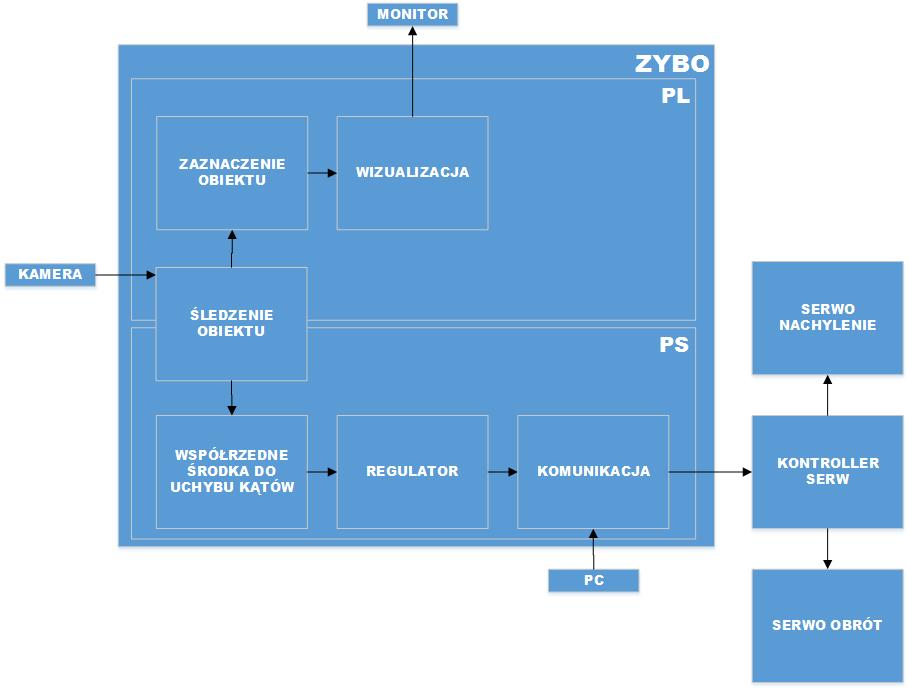
\includegraphics[width=4in]{scheme_pol.jpg}
	\caption{Schemat realizowanego rozwiązania.}
	\label{fig:schemat}
\end{figure}

Pracę postanowiono podzielić na kilka niezależnych modułów. Na rysunku \ref{fig:schemat} przedstawiono ten podział oraz połączenia między modułami.
\begin{itemize}
\item Śledzenie obiektu - zawiera elementy odpowiedzialne za odbiór i dekodowanie danych z kamery. Oprócz tego zawiera właściwy algorytm śledzenia. Wyjściami tego segmentu są odpowiednio opóźnione sygnały wejściowe, współrzędne wyznaczonego punktu oraz sygnał oznaczający obliczenie nowych współrzędnych.
\item Zaznaczenie obiektu - zaznacza w ramce otrzymane współrzędne. Zaznaczenie może mieć postać dwóch prostopadłych linii lub prostokąta.
\item Wizualizacja - odpowiada za kodowanie danych z postaci RGB i sygnałów synchronizacyjnych do postaci VGA oraz wysłanie ich.
\item Współrzędne środka do uchybu kątów - przelicza współrzędne wejściowe do postaci uchybu kątów nachylenia i obrotu.
\item Regulator - na podstawie uchybów kątów otrzymanych na wejściu oblicza pozycje zadane dla serwomechanizmów, przelicza je na szerokości impulsów i przekazuje je na wyjście.
\item Komunikacja - odpowiada za odbieranie poleceń i danych z komputera PC oraz wysyłanie odpowiednich do sterownika serwomechanizmów. Jeśli włączony jest tryb pracy autonomicznej, to szerokość impulsów otrzymaną z regulatora do sterownika.
\end{itemize}

\section{Zawartość pracy}
\label{sec:zawartoscpracy}

%TODO Sugeruje jednak albo wypunktowanie, albo tekst ciągły. -zmienione.

\begin{itemize}
\item W rozdziale drugim wykonano przegląd algorytmów śledzenia i dokonano wyboru algorytmu do implementacji w sprzęcie.
\item W rozdziale trzecim opisano skompletowane stanowisko. Przedstawiono specyfikację użytych elementów oraz uzasadniono ich wybór.
\item W rozdziale czwartym scharakteryzowano komunikację pomiędzy elementami realizowanego systemu (PC-Zynq-Maestro).
\item W rozdziale piątym opisano model matematyczny sterowanego obiektu oraz projekt implementowanego regulatora. Krótko omówiono wynik testu regulatora na modelu.
\item W rozdziale szóstym opisano podstawowy tor wizyjny, otrzymujący obraz z kamery i wysyłający go bez zmian na wyjście. Przedstawiono realizację algorytmu śledzenia przez detekcję.
\item W rozdziale siódmym przedstawiono implementację w platformie sprzętowej gotowego algorytmu Mean-shift, wykonanego przez pana Krzysztofa Mazura w ramach koła naukowego \textit{AVADER}.
%TODO Lepiej , że p. Krzysztofa Mauzura w ramach AVADER. -zrobione.
%TODO nie podoba mi się słowo zrealizowne -zrobione.
%TODO A nie ma śledznia przez detekcję. -dodano do rozdziału szóstego.
\item W rozdziale ósmym przeprowadzono próbę implementacji algorytmu KLT. Opisano działanie modułów odpowiedzialnych za wyznaczanie punktów charakterystycznych obrazu oraz przedstawiono ich działanie na przykładzie.
%TODO Do ew. aktualizacji
\item W rozdziale dziewiątym podsumowano wykonane zadania. Omówiono wnioski na podstawie przeprowadzonych prac. Przedstawiono zadania, które zostaną zrealizowane w przyszłości.
\end{itemize}